\begin{figure*}[h!]
    \centering
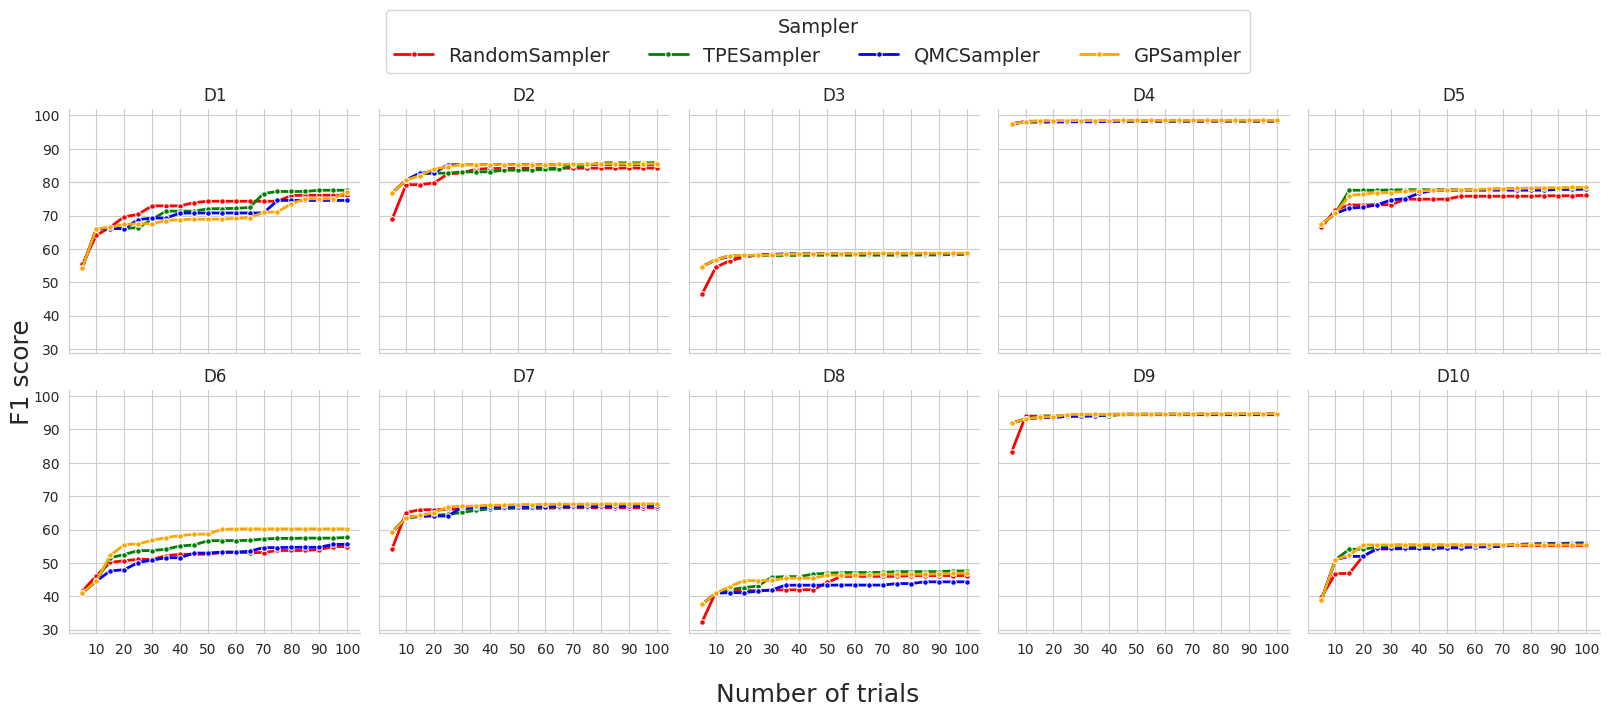
\includegraphics[width=0.97\textwidth]{figures/predictions/f1_convergence_plots.png}
    % \vspace{-10pt}
    \caption{F1-score of the sampling-based search algorithms in Section \ref{sec:problem-1} as the number of trials increases from 5 to 100.}
    \label{fig:samplers-convergence-avg-f1}
\end{figure*}

\section{Experimental Evaluation - Problem 1}\label{sec:experiments-p1}
%In this section, we first present our experiments for tackling Problem~\ref{pr:pr1} (Section~\ref{sec:problem-1}), and then by utilizing all the results produced we proceed on showing the results for tackling Problem~\ref{pr:pr2} (Section~\ref{sec:problem-2}).


%\begin{figure}[t]
%    \centering
%    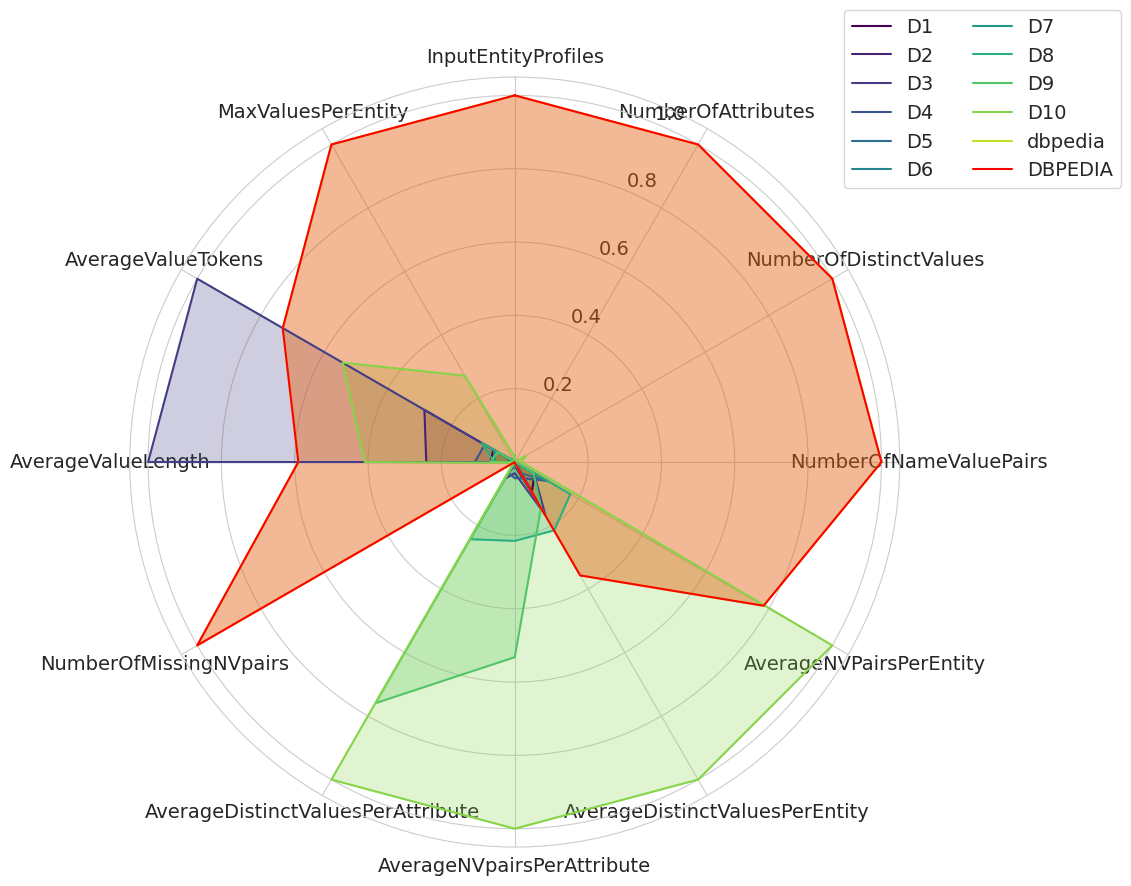
\includegraphics[width=\linewidth]{figures/predictions/dataset_specs_radar.png}
%    \caption{All dataset features comparison.}
%    \label{fig:datasets-radar}
%\end{figure}

\begin{table}[t]
\centering 
\small 
\caption{Technical characteristics of the datasets used in our experimental analysis. $|E_x|$ stands for the number of entities in data source $x$ and $|D|$ for the number of duplicates. 
} 
\label{tab:dataset-specs}
\begin{tabular}{|p{0.9cm}|p{2.1cm}|r|r|r|}
\hline
\multicolumn{1}{|c|}{\textbf{Dataset}} & \multicolumn{1}{|c|}{\textbf{Names}} & \multicolumn{1}{|c|}{\textbf{$\mathbf{|E_1|}$}} & \multicolumn{1}{|c|}{{$\mathbf{|E_2|}$}} & \multicolumn{1}{|c|}{\textbf{$\mathbf{|D|}$}} \\
\hline
\hline
\multirow{2}{*}{D1} & Restaurants1-& \multirow{2}{*}{340} & \multirow{2}{*}{2,257} & \multirow{2}{*}{89} \\
& Restaurants2 & & & \\
\hline
D2 & Abt-Buy & 1077 & 1,076 & 1,076 \\
\hline
\multirow{2}{*}{D3} & Amazon- & \multirow{2}{*}{1,355} & \multirow{2}{*}{3,040} & \multirow{2}{*}{1,103} \\
& Google Products & & & \\
\hline
D4 & DBLP-ACM & 2,617 & 2,295 & 2,225 \\
\hline
D5 & IMDB-TMDB & 5,119 & 6,057 & 1,969 \\
\hline
D6 & IMDB-TVDB & 5,119 & 7,811 & 1,073 \\
\hline
D7 & TMDB-TVDB & 6,057 & 7,811 & 1,096 \\
\hline
\multirow{2}{*}{D8} & Walmart- & \multirow{2}{*}{2,555} & \multirow{2}{*}{22,075} & \multirow{2}{*}{853} \\
& Amazon & & & \\
\hline
D9 & DBLP-Google Scholar & 2,517 & 61,354 & 2,309 \\
\hline
D10 & IMDB-DBpedia & 27,616 & 23,183 & 22,864 \\
\hline
\hline
D11 & DBpedia & 1,190,734 & 2,164,041 & 892,579 \\
\hline
\end{tabular}
\end{table}

\subsection{Experimental setup}
\label{sec:expSetup}
All experiments were implemented in Python, v. 3.9. For the implementation of the ETEER pipeline, we used pyJedAI v. 0.1.8\footnote{\underline{https://github.com/AI-team-UoA/pyJedAI}}. 
%To tackle Problem 1, 
For the implementation of the sampling algorithms, we used Optuna v. 3.6.1\footnote{\underline{https://optuna.org}}. 
%: 4381MiB / 128831MiB.
All 
%Optuna,  Linear Regression approach and
%Trials, \& DL (in general pyJedAI)
%pyJedAI 
experiments 
%for that problem 
were executed on a server running 
%executed on [OS: 
Ubuntu 22.04, 
%equipped 
with Intel Core i7-9700K @4,9GHz and 68 GB RAM.
%: 6622MiB / 64228MiB]
%D11 experiment was executed in the same server.

%\textbf{Evaluation.} The evaluation metrics include mean squared error (MSE), the ratio of the best-predicted F1-score to the \textit{global maximum F1}-score. After exploring all Optuna and Grisearch trials, the maximum F1-score per dataset, serves as the global best F1-score (GB-F1). Also, for the evaluation of the predicted configurations we measured the difference between the predicted and actual best scores. Specifically, this metric will be found later as \textit{Performance} and it is the fraction of ETEER predicted configuration F1 divided by the GB-F1 for each dataset.


\textbf{Datasets.} For Record Linkage, we use 11 publicly available, real-world datasets that are popular in the literature~\cite{DBLP:journals/pvldb/Thirumuruganathan21,DBLP:journals/pvldb/KopckeTR10,DBLP:conf/sigmod/MudgalLRDPKDAR18}. Their technical characteristics are reported in Table~\ref{tab:dataset-specs}. $D_{1}$, which was first used in OAEI 2010,
%\footnote{\underline{http://oaei.ontologymatching.org/2010}}, 
contains restaurant descriptions. $D_{2}$ encompasses duplicate products from the online retailers Abt.com and Buy.com \cite{DBLP:journals/pvldb/KopckeTR10}. $D_{3}$ matches product descriptions from Amazon.com and the Google Base data API (GB) \cite{DBLP:journals/pvldb/KopckeTR10}. $D_{4}$ entails bibliographic data from DBLP and ACM \cite{DBLP:journals/pvldb/KopckeTR10}. $D_{5}$, $D_{6}$ and $D_{7}$ involve descriptions of television shows from TheTVDB.com (TVDB) and of movies from IMDb and themoviedb.org (TMDb) \cite{DBLP:conf/esws/ObraczkaSR21}. $D_{8}$ matches product descriptions from Walmart and Amazon \cite{DBLP:conf/sigmod/MudgalLRDPKDAR18}. $D_{9}$ involves bibliographic data from publications in DBLP and Google Scholar (GS) \cite{DBLP:journals/pvldb/KopckeTR10}. Finally, 
$D_{10}$ interlinks movie descriptions from IMDb and DBpedia \cite{DBLP:journals/vldb/PapadakisETHC23}, including a different snapshot of IMDb than $D_5$~and~$D_6$. 
% Finally, D11 matches two different versions of DBpedia that chronologically differ by 3 years \cite{DBLP:journals/is/PapadakisMGSTGB20}. 

% Note that D11 is only used to address RQ3 in Section \ref{sec:expProblem2}, unlike the other datasets, which are used in all other experiments.
%Figure \ref{fig:datasets-radar} explores the dataset features extracted from each dataset, illustrating that D2 through D6 exhibit similar feature values, whereas D8, D9, D10, and particularly D11 differ significantly, with D11 representing a completely distinct feature area.

%{\color{red}Explain that D11 is used only in Problem 2 and why.}

%{\color{red} The training data was preprocessed by scaling and converting categorical variables into dummy variables to maintain consistency across all datasets. WHERE SHOULD THIS SENTENCE GO? Vasilis: mallon pouthena `h estw sto github}

\begin{table*}[t]
\begin{center}  
\small 
\caption{Performance of the two baseline methods for Problem 1: (a) the default workflow (st5, 10, UniqueMappingClustering, 0.5), and (b) the best grid-search trial. For the latter, we also report the parameter configuration.}
\label{tab:best-gridesearch-trials}
\begin{tabular}{|c||c|c||c|c|c|c||c|c|c|}
\hline
\multirow{2}{*}{Dataset} & \multicolumn{2}{c||}{Default configuration} & \multicolumn{7}{c|}{Best grid-search configuration} \\
& F1-score & Runtime (sec) & LM & K & Clustering & Threshold & F1-score & Runtime (sec) & Grid search time (hrs) \\
\hline
\hline
D1 & 47.44 & 1.90 & smpnet & 3 & CCC & 0.90 & 75.53 & 2.87 & 41 \\
D2 & 85.85 & 3.28 & st5 & 10 & UMC & 0.35 & 85.85 & 2.51 & 38 \\
D3 & 57.35 & 1.49 & sminilm & 7 & UMC & 0.45 & 59.19 & 1.43 & 45 \\
D4 & 97.56 & 4.45 & st5 & 1 & UMC & 0.80 & 98.60 & 1.43 & 45 \\
D5 & 57.74 & 5.05 & st5 & 6 & KC & 0.75 & 78.73 & 2.98 & 60 \\
D6 & 30.39 & 1.81 & sminilm & 1 & UMC & 0.55 & 60.25 & 0.91 & 71 \\
D7 & 35.68 & 2.21 & sminilm & 93 & CCC & 0.80 & 67.36 & 28.64 & 74 \\
D8 & 35.82 & 4.46 & st5 & 4 & KC & 0.90 & 47.56 & 3.19 & 145 \\
D9 & 92.04 & 13.11 & st5 & 42 & KC & 0.80 & 94.89 & 21.37 & 329 \\
D10 & 53.63 & 27.96 & st5 & 2 & KC & 0.65 & 56.12 & 28.77 & 320 \\
\hline
\end{tabular}
% \vspace{-8pt}
\end{center}  
\end{table*}

\subsection{Evaluation Results}
\label{sec:tackleProblem1}
We address three research questions while tackling Problem~1:
\begin{enumerate}[leftmargin=*, label=RQ\arabic*), start=1]
    \item Which of the sampling-based search algorithms 
    %of those discussed 
    in Section \ref{sec:problem-1} converges faster 
    %i.e., with fewer trials, 
    to its maximum performance?
    \item Does sampling-based search outperform the baselines with respect to effectiveness?
    \item Does sampling-based search outperform the baselines with respect to time efficiency?
\end{enumerate}

We use two approaches as baselines: 
\begin{enumerate}[leftmargin=*]
    \item A default configuration based on \cite{DBLP:journals/pvldb/ZeakisPSK23} that combines the s-t5 language model with $k$=10, Unique Mapping Clustering and similarity threshold = 0.5. 
    %The performance of this baseline method is reported in Table \ref{???}.
    \item The best performance estimated by grid search among the configuration parameters in Table \ref{tab:parameter-values}. %The corresponding performance is reported in Table \ref{tab:best-gridesearch-trials}.
\end{enumerate}

The performance of those baselines per dataset with respect to effectiveness and time efficiency is reported in Table~\ref{tab:best-gridesearch-trials}.

\textbf{RQ1.}
We evaluate all samplers discussed in Section~\ref{sec:problem-1}, configuring each one 
%\textit{TPESampler}, \textit{RandomSearchSampler}, \textit{QMCSampler}, and \textit{GPSampler}. Optuna was configured 
to run 100 trials per dataset, according to the recommendations from the Optuna documentation\footnote{\underline{https://optuna.readthedocs.io/en/stable/reference/samplers/index.html}}. To analyze the convergence behavior of each sampler, we vary the maximum number of trials from 5 to 100, in increments of 5. For each budget of trials, we perform experiments with five different random seeds and consider the average, thus providing a robust estimation of the actual performance per number of trials. The results appear in Figure \ref{fig:samplers-convergence-avg-f1}, with the horizontal axes corresponding to the number of trials and the vertical ones to the respective average F1-score.

%The objective was to determine the number of trials needed to find a near-optimal solution. Figure \ref{fig:samplers-convergence-avg-f1} illustrates the convergence analysis of each sampler across all datasets. The y-axis shows the average of the maximum F1-scores achieved per sampler. This "maximum" refers to the highest F1-score within each set of trials (5, 10, ..., 100), and the "average" is computed across five different random seeds, providing an average of these maximum scores. The x-axis represents the different sets of trials evaluated. 

%The number of trials in Optuna is a user-defined parameter, and Optuna will execute exactly the number of trials specified. 
For all samplers, convergence is generally observed in around 30 trials for most datasets. This means that with just 30 trials, they approximate the best performance in almost all datasets.
%μαπaccompanied by a complete ground truth. 
The only exceptions are $D_1$, $D_6$ and $D_8$. As observed in Figure \ref{fig:f1_boxplot_all}, in these datasets the portion of configuration parameters that maximize F1 is rather small. As a result, we need to increase the number of trials to much more than 30 in order to identify a configuration matching or approximating the maximum performance.

Regarding the relative performance of the considered samplers, Figure \ref{fig:samplers-convergence-avg-f1} indicates that there are no significant differences among them. Their behavior is quite similar, determined largely by the dataset at hand. Nevertheless, \textit{GPSampler} shows marginally better results in several cases.

\textbf{RQ2.} We now compare the effectiveness of the four samplers with that of the two baselines in Table \ref{tab:best-gridesearch-trials}. 
For the grid-search baseline, we also report the best-performing configuration.
%and the total time taken to run the grid search.
As expected, the default configuration consistently underperforms grid search to a significant extent. The only exception appears in $D_2$, where they yield the same F1-score, because the grid search configuration is almost identical with the default one (they differ only in the similarity threshold). Hence, for brevity, we exclusively compare the samplers with the best grid search configuration.

%To benchmark the Optuna approach, we also conducted an exhaustive grid search for each dataset. The search space explored is detailed in Table \ref{tab:parameter-values}, where the Cartesian product of all parameters results in a total of $7 \times 3 \times 19 \times 100 = 39,900$ possible configurations. 
%\comments{giati to leme edw? pws sundeetai me tin panw paragrafo? giati xreiazetai na to kseroume? mia protasi akoma xreiazetai.}

%\begin{figure*}[h!]
%    \centering
%    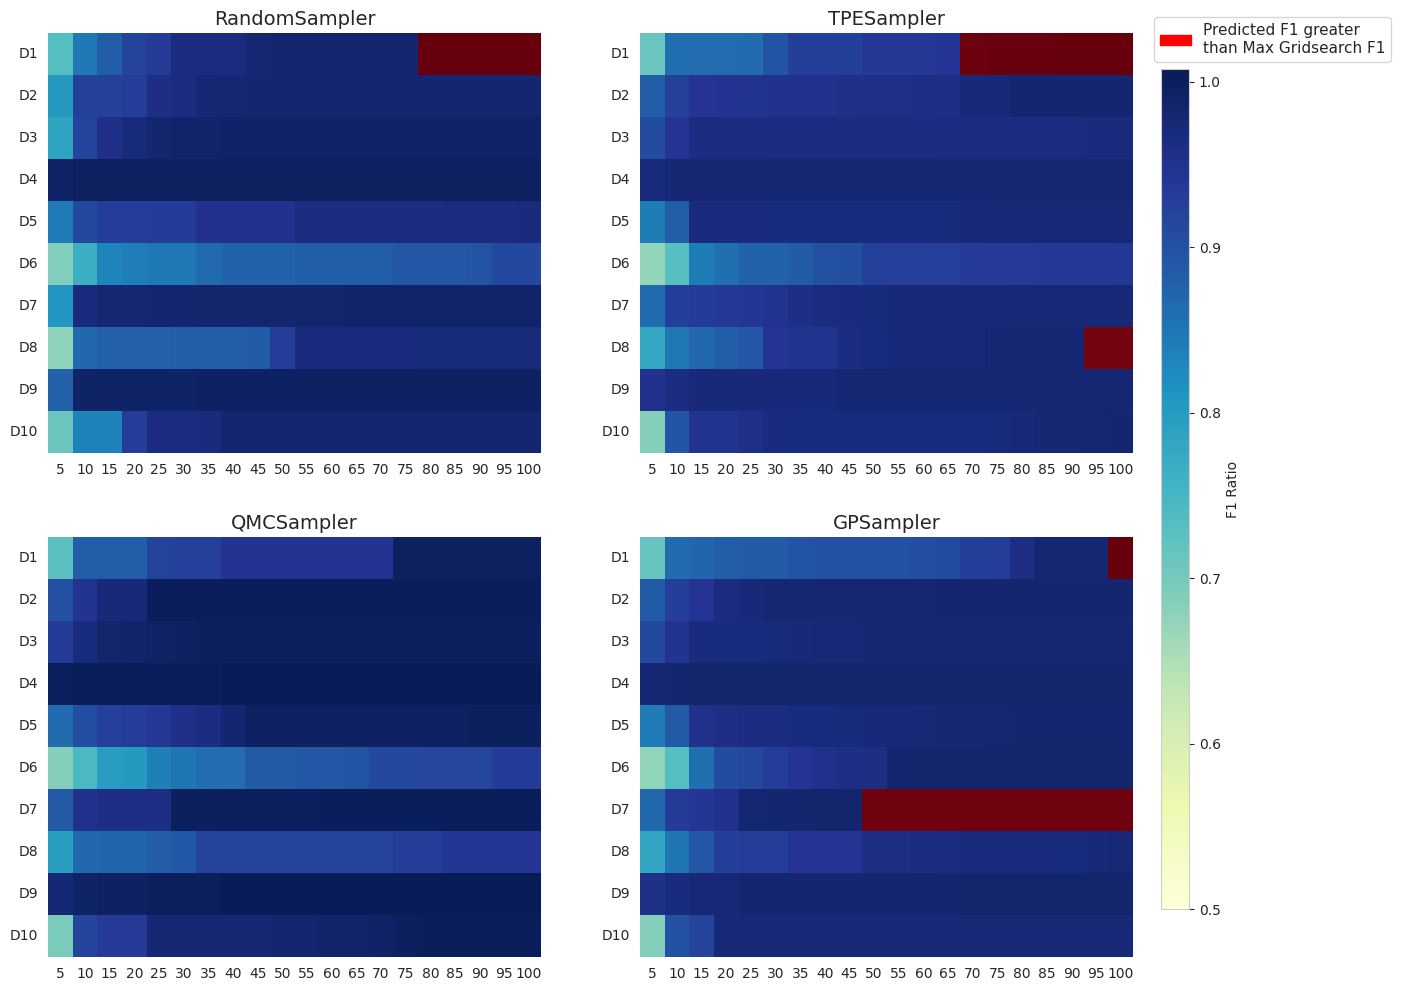
\includegraphics[width=0.97\textwidth]{Nikoletos-paper/figures/predictions/sampler_heatmaps.png}
%    \caption{Samplers F1-Ratio heatmaps.}
%    \label{fig:samplers-heatmaps-f1}
%\end{figure*}

% \begin{figure*}[t]
%     \centering
%     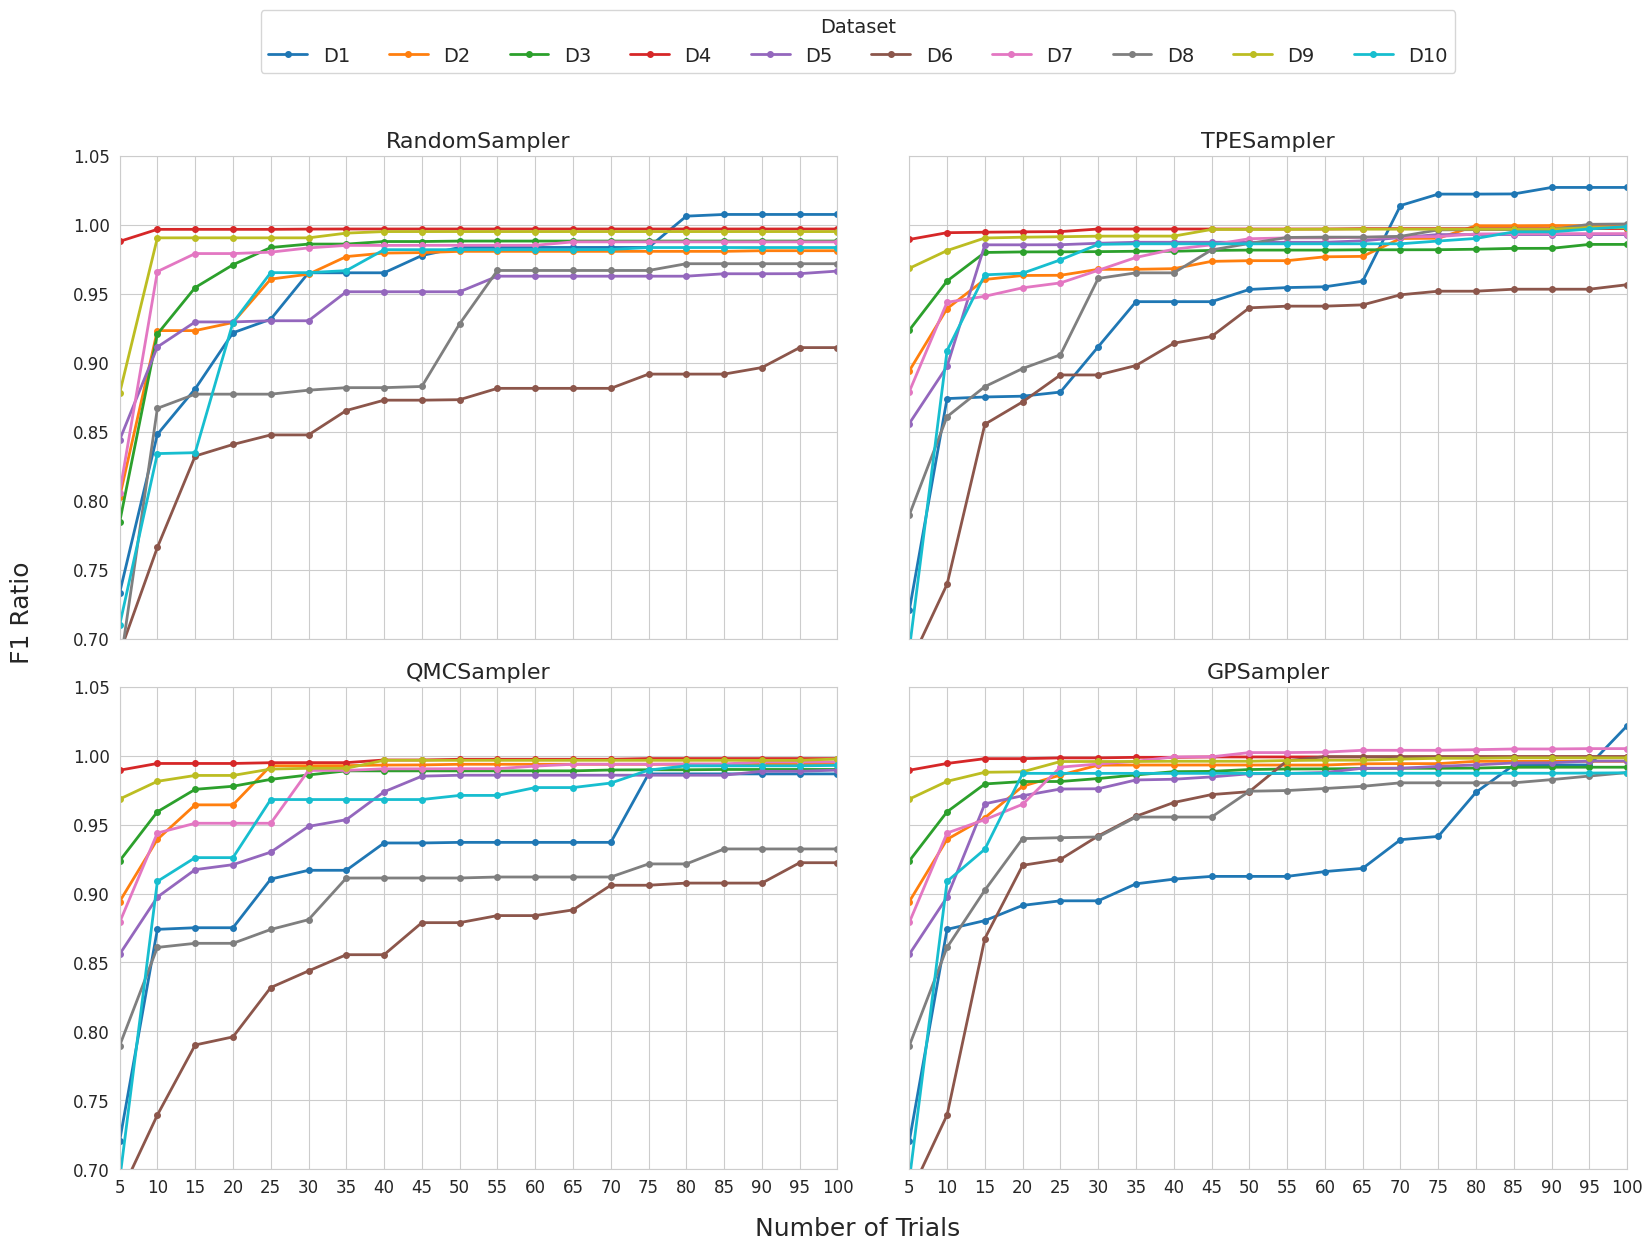
\includegraphics[width=0.8\textwidth]{Nikoletos-paper/figures/predictions/f1_ratio_vs_trials_subplots.png}
%     \vspace{-10pt}
%     \caption{The ratio between the F1-score of the sampling-based search algorithms and the F1-score of grid search.}
%     \label{fig:p1-samplers-performance-f1}
%     %\vspace{-10pt}
% %\end{figure*}

% %\begin{figure*}[t]
%     \centering
%     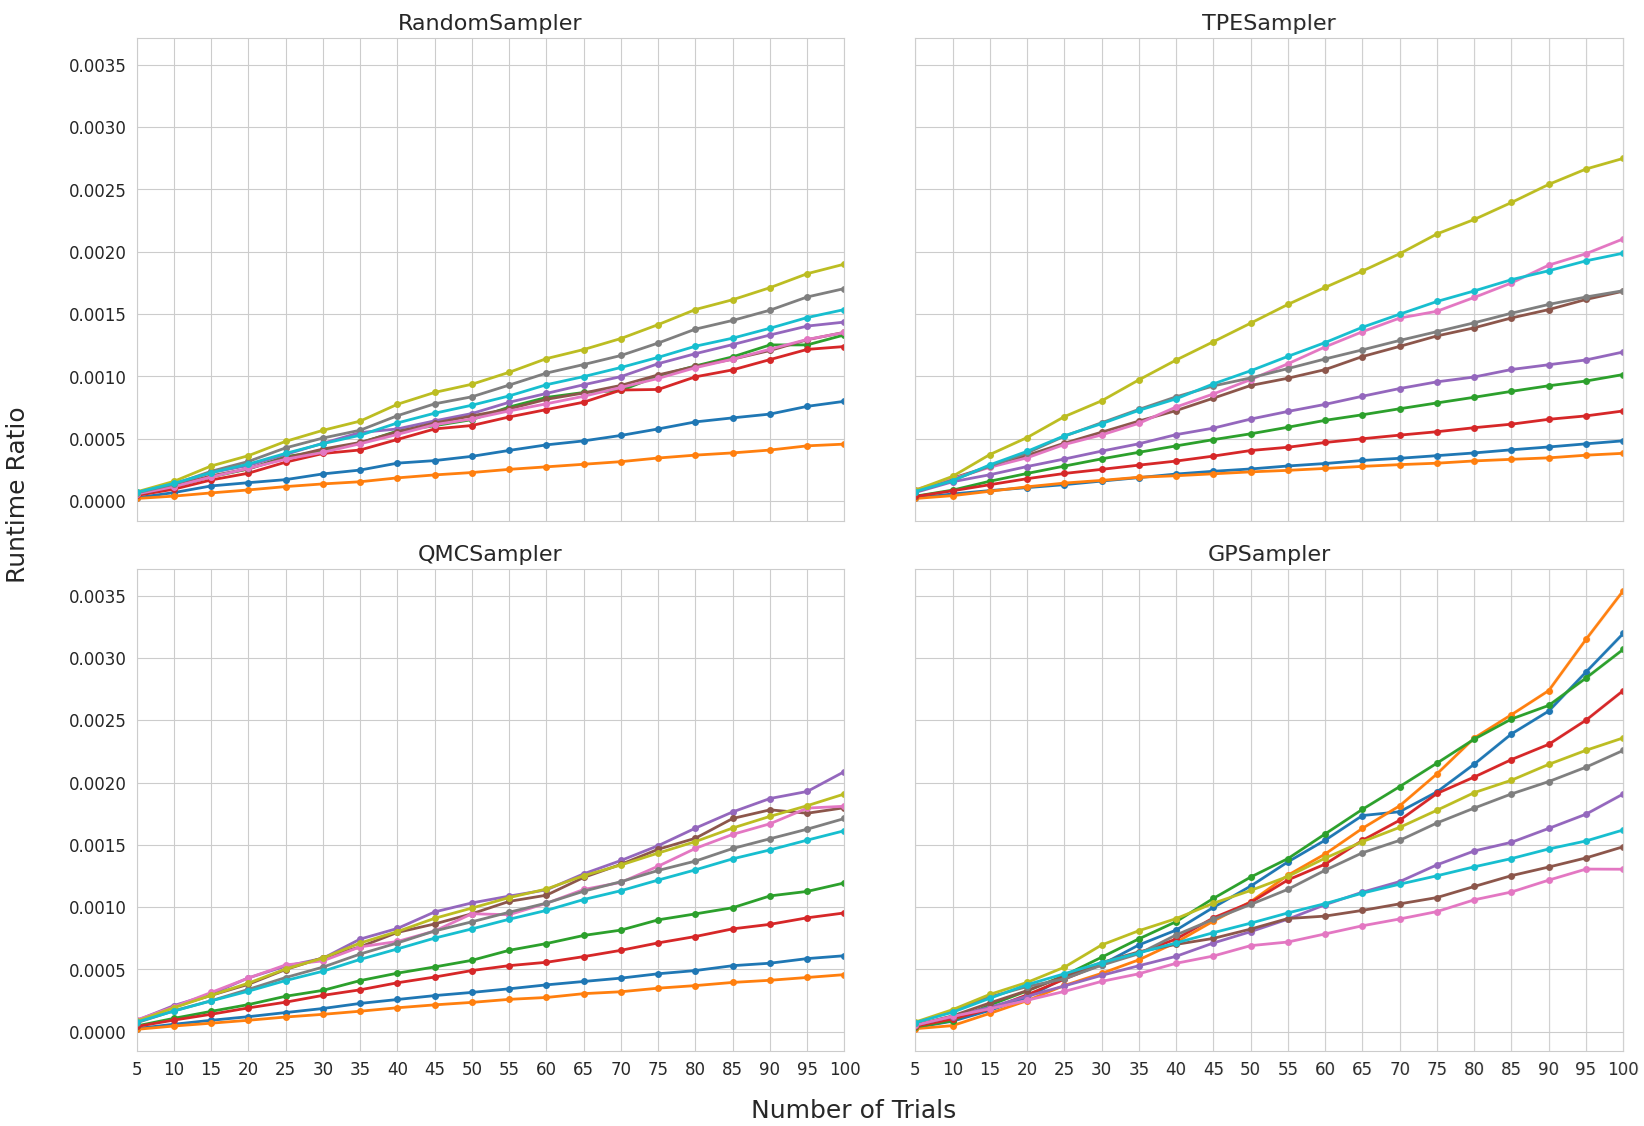
\includegraphics[width=0.8\textwidth]{Nikoletos-paper/figures/predictions/runtimes_ratio_vs_trials_subplotsV2.png}
%     \vspace{-10pt}
%     \caption{The ratio between the run-time of the sampling-based search algorithms and the run-time of grid search.}
%     \label{fig:p1-samplers-performance-runtimes}
%     \vspace{-10pt}
% \end{figure*}

\begin{figure*}[t]
    \centering
    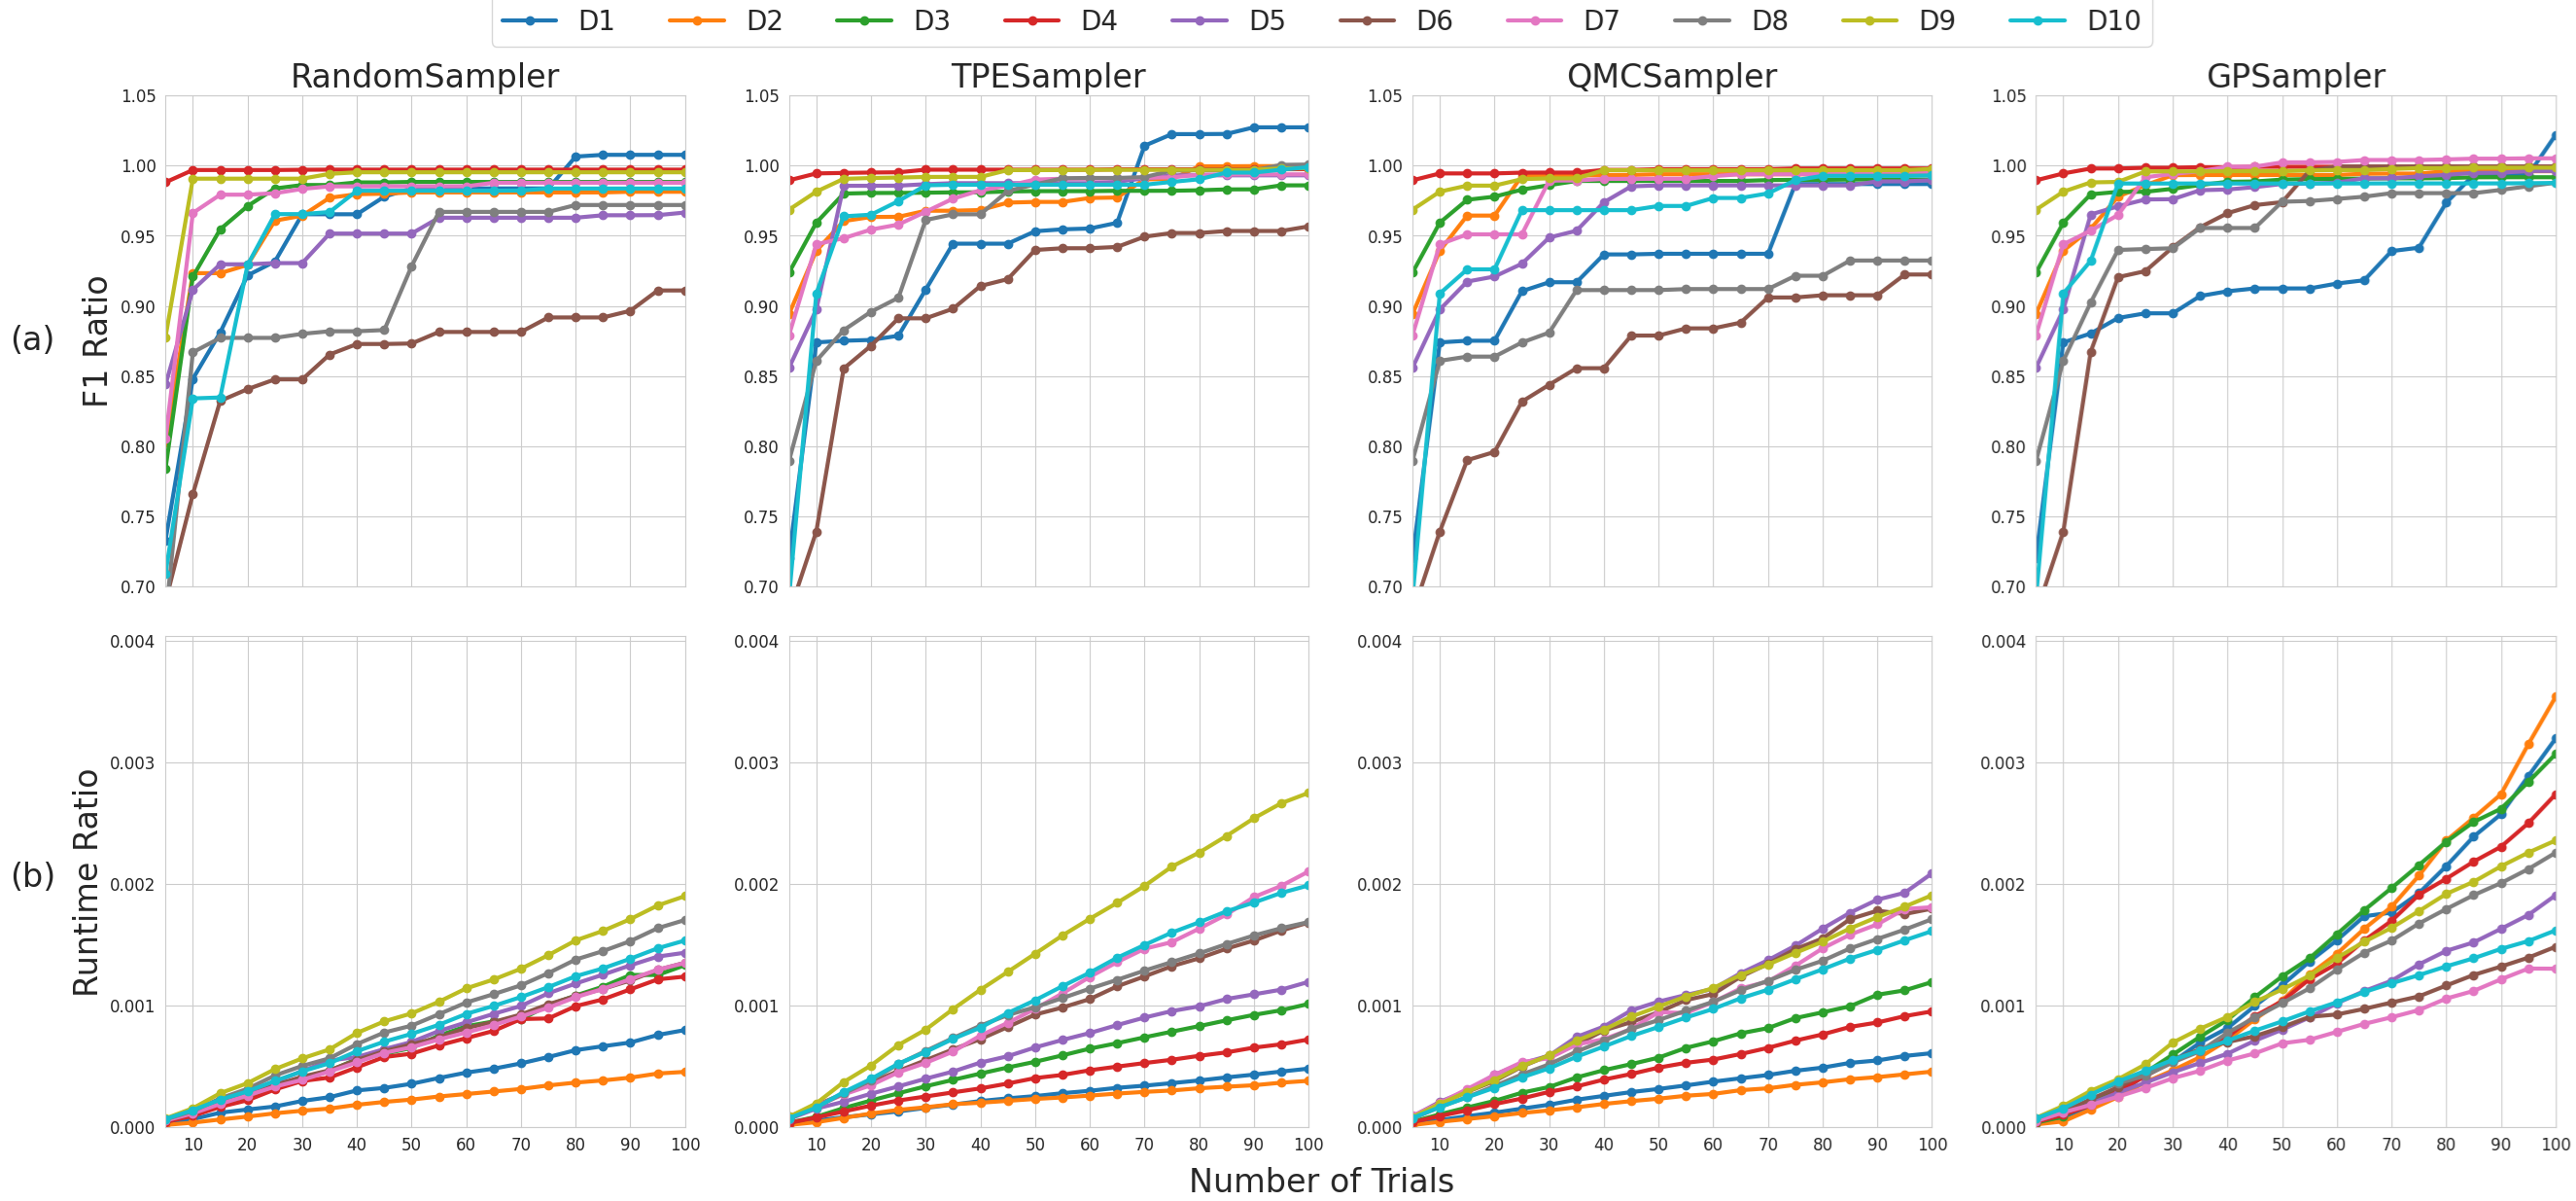
\includegraphics[width=0.99\textwidth]{Nikoletos-paper/figures/predictions/combined_f1_runtime_ratios_vs_trials.png}
    % \vspace{-10pt}
    \caption{The ratio between (a) the F1-score of sampling-based search algorithms and grid search, and (b) their run-times.
    %algorithms and the F1-score/Runtime of grid search.
    }
    \label{fig:p1-samplers-performance-f1}
\end{figure*}

This comparison is depicted in Figure \ref{fig:p1-samplers-performance-f1}(a), which contains a separate diagram for each sampler with its convergence to the best grid search performance in Table \ref{tab:best-gridesearch-trials}. The vertical axes 
%in Figure \ref{fig:p1-samplers-performance-f1} 
correspond to \textit{F1 ratio}, which is defined as ``samplerF1''/``gridSearchF1''. That is, an F1 ratio of 1.0 indicates that the two approaches yield the same F-Measure despite their different configuration. Values lower than 1.0 indicate lower sampling-based performance than grid search, while ratios $>1.0$ denote that the sampler identified a configuration that outperforms all those tested by grid search. This should be attributed to the discrete similarity thresholds considered by grid search, unlike samplers, which may consider any value in $[0,1]$.

%We observe that the 
RandomSampler underperforms grid search in almost all cases. Yet, with just 20 trials, its F1 ratio exceeds 0.90 in all datasets but
%is less than 10\% lower than the best one of grid search, except for 
$D_1$, $D_6$ and $D_8$.
These three datasets 
convey very few top-performing configurations, as shown in Figure \ref{fig:f1_boxplot_all}. 
%RandomSampler 
%reaches 95\% of grid search's F1 
Note also that with just 30 trials, its F1 ratio exceeds 0.95 in all datasets but $D_1$, $D_6$ and $D_8$. In $D_1$, RandomSampler converges to grid search after 70 trials, outperforming it to a minor extent after 80 trials, while in $D_6$ and $D_8$, its F1 ratio raises up to 0.93 after 100 trials, because there is an even lower portion of top-performing configurations. 

TPESampler exhibits a much 
%better 
quicker
convergence. With only 20 trials, its F1 ratio is higher than 0.95 in all datasets but the most challenging ones, namely $D_1$, $D_6$ and $D_8$. For 30 trials, its F1 ratio is lower than 0.95 only in two datasets: $D_1$ and $D_6$. In $D_1$, TPESampler outperforms grid search by $\sim$2.5\% after just 65 trials, while in $D_6$, its F1 ratio exceeds 0.95 after 70 trials. 

QMCSampler exhibits a performance similar to RandomSampler. After 20 trials, its F1 ratio is lower than 0.90 in only two datasets: $D_6$ and $D_8$. After 30 trials, its F1 ratio is lower than 0.95 in three datasets: $D_5$, $D_6$ and $D_8$. For the first two of these datasets, it matches the effectiveness of grid search after 55 trials, but its F1-score in $D_8$ is almost 9\% lower than grid search after 100 trials. In $D_1$, QMCSampler converges faster than all other samplers, with its F1 ratio exceeding 0.95 after 30 trials and 1.00 
%while outperforms grid search 
after 80 trials. 

Finally, GPSampler is similar to TPESampler. After 20 trials, its F1 ratio exceeds 0.95 in all but the three most challenging datasets, i.e., $D_1$, $D_6$ and $D_8$. For the last two, the F1 ratio raises to 0.94 after 30 trials, with $D_1$ converging much slower, after 80 trials, eventually outperforming grid search after 100 trials. The same applies to a minor extent to $D_7$, too. Note also that GPSampler is the only approach that matches or exceeds the performance of grid search across all datasets after 100 trials. Hence, it is considered the top performing approach, albeit to a minor extent in most cases.

\begin{table}[t]
\centering
\small 
\setlength{\tabcolsep}{2.5pt}
\caption{The highest F1-score among the configurations considered by the sampling-based search algorithms in Section~\ref{sec:problem-1}.}
\label{tab:global-bestf1s}
\begin{tabular}{|c|c|c|c|c|c|c|r|}
\hline
Dat. & LM & k & Clustering & Threshold & Sampler & F1 & RT (s) \\
\hline
\hline
D1 & st5 & 73 & CCC & 0.874280 & tpe & 78.43 & 0.95 \\
D2 & st5 & 10 & UMC & 0.594537 & tpe & 85.85 & 0.38 \\
D3 & sminilm & 10 & UMC & 0.429178 & random & 58.97 & 0.43 \\
D4 & st5 & 1 & UMC & 0.759879 & gps & 98.56 & 6.58 \\
D5 & st5 & 1 & CCC & 0.765179 & gps & 78.92 & 3.67 \\
D6 & sminilm & 1 & UMC & 0.555229 & gps & 60.42 & 1.30 \\
D7 & sminilm & 84 & CCC & 0.811881 & gps & 67.76 & 5.22 \\
D8 & st5 & 75 & KC & 0.920773 & tpe & 49.53 & 6.45 \\
D9 & st5 & 65 & KC & 0.830563 & tpe & 94.92 & 16.83 \\
D10 & st5 & 2 & KC & 0.269090 & tpe & 56.11 & 14.03 \\
\hline
\end{tabular}
\end{table}


\textbf{RQ3.} To estimate the relative time efficiency of grid and sampling-based search, we define the \textit{runtime ratio} as $rt(sa, n)/rt(gs)$, where $rt(sa, n)$ stands for the overall run-time required by each sampler for $n$ trials, on average, across the 5 iterations (based on different seeds), and $rt(gs)$ for the overall run-time required by grid-search for the same dataset, as reported in Table \ref{tab:best-gridesearch-trials} -- $rt(sa, n)$ and $rt(gs)$ involve both the time required for generating the next parameter configuration to be tested and the run-time of the corresponding ETEER pipeline. The runtime ratio is defined in $[0,1]$, with values $<1$ indicating 
%higher time efficiency, i.e.,
that sampling-based is faster than grid search. 

The actual values of the runtime ratio per sampler, dataset and number of trials is depicted in Figure \ref{fig:p1-samplers-performance-f1}(b). We observe that in all cases, its value is well below 0.35\%. This means sampling-based search is consistently faster than grid search by more than 285 times. Typically, the larger a dataset is, the higher is the runtime ratio, because of the more time-consuming ETEER pipelines that have to be evaluated. The relative run-time of the sampling-based algorithms is determined by their relative time complexity: the fastest approach is RandomSampler followed in close distance by QMCSampler, given their time complexity, $O(d)$ and $O(d n)$, resp.; TPESampler is consistently slower, $O(d n logn)$, with GPSampler exhibiting the highest run-times, due to its cubic time complexity.

\begin{figure}[t]
    \centering
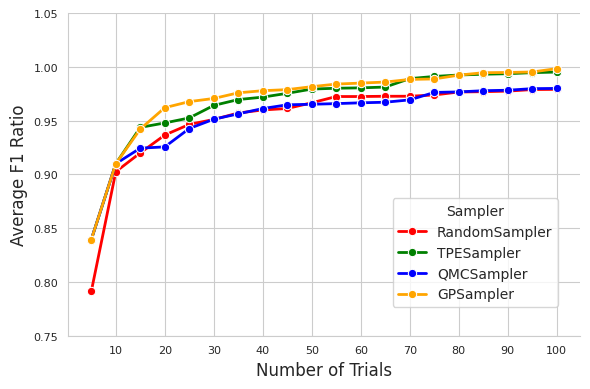
\includegraphics[width=0.97\linewidth]{Nikoletos-paper/figures/predictions/average_f1_ratios_across_datasets.png}
    % \vspace{-10pt}
    \caption{Average F1 score per sampler and per trial, across all the datasets.}
    \label{fig:mean-F1-samplers-performance-f1}
\end{figure}

\textbf{Conclusions.} We can conclude that all considered sampling-based search algorithms for parameter fine-tuning are capable of approximating the performance of grid search in any of the considered datasets, while being faster by at least 2 orders of magnitude.
%despite using 399 times less trials. 
The larger the portion of top-performing configurations in a dataset, the fewer trials are needed by these algorithms. Nevertheless, they consistently underperform grid search, albeit to an insignificant extent ($\ll0.5\%$).
%Note, though, that they rarely outperform grid search: 
Comparing their best performance in Table~\ref{tab:global-bestf1s} with the best grid search one in Table~\ref{tab:best-gridesearch-trials}, we observe that only in $D_1$ and $D_8$ the former outperforms the latter by 2\%-3\%. {Overall, though, the difference between the two approaches is statistically insignificant ($p=0.13437$) (unlike the difference between the default configuration in Table~\ref{tab:best-gridesearch-trials} and the best sampling performance in Table~\ref{tab:global-bestf1s}).}
%-- in all other cases, their difference is statistically insignificant . 
As a result, sampling-based search basically 
%thus offering a much faster approach to approximating grid search.
%Overall, we can conclude that the sampling-based algorithms for parameter fine-tuning 
offers a much better balance between effectiveness and time efficiency than grid search: for the same F1 score, the number of trials and the corresponding run-time is reduced by 2 or even 3 orders of magnitude. Among the sampling-based algorithms, the fastest convergence and the highest effectiveness typically correspond to GPSampler, especially for 20-30 trials, as shown in Figure \ref{fig:mean-F1-samplers-performance-f1}, which estimates the average F1 per number of trials for each sampler across all datasets in Table~\ref{tab:dataset-specs}. {Note that the superiority of GPSampler over the other three samplers is statistically significant ($p\ll0.05$) in Figure~\ref{fig:mean-F1-samplers-performance-f1}}.

